\documentclass[12pt]{beamer}
\usepackage[utf8]{inputenc}
\usepackage[T1]{fontenc}
\newif\ifpt
\usepackage{user}
\ifpt
\usepackage[portuguese]{babel}
\else
\usepackage[english]{babel}
\fi
\usepackage{graphicx}
\usepackage{color}

\colorlet{mybasecolor}[rgb]{blue!60!black}
\usepackage{slidesdef}

\author{\autor}
\title{\titulo}
\date{\data}

\begin{document}

\myframe{
  \begin{beamercolorbox}[center, rounded=true, shadow=true]{mainbox}
    \bf \LARGE \titulo
  \end{beamercolorbox}
  \hfill
  \begin{beamercolorbox}[center, wd=0.8\textwidth, rounded=true,
      shadow=true]{secbox}
    \bf \large \evento
  \end{beamercolorbox}
  \hfill{}

  \linespread{1.0}
  \begin{center}
    \textbf{\autor}
    \vspace{-4pt}
    {\scriptsize \\ \instautor}
    \ifdefined\colabum
      \vspace{10pt}
      \textbf{\\ \colabum}
      \vspace{-4pt}
      {\scriptsize \\ \instcolabum}
    \fi
    \ifdefined\colabdois
      \vspace{10pt}
      \textbf{\\ \colabdois}
      \vspace{-4pt}
      {\scriptsize \\ \instcolabdois}
    \fi
    \ifdefined\colabtres
      \vspace{10pt}
      \textbf{\\ \colabtres}
      \vspace{-4pt}
      {\scriptsize \\ \instcolabtres}
    \fi
    \ifdefined\colabquatro
      \vspace{10pt}
      \textbf{\\ \colabquatro}
      \vspace{-4pt}
      {\scriptsize \\ \instcolabquatro}
    \fi
    {\small \\ \vfill \data}
  \end{center}
}

\begin{frame}
  \tableofcontents
\end{frame}

\section{Zeros de Funções}
\subsection{Introdução}

\AtBeginSection[]
{
 \begin{frame}<beamer>
   \tableofcontents[currentsection]
 \end{frame}
}


\myframe{
  \ctr{ Zeros de uma função real }
  \only<1>{
  \[ f(x) = 0, \qquad f:\mathbb{R}\rightarrow\mathbb{R} \]
  }
  \only<2->{
  \[ f(x) = (x^2-1)(x^2-4) + \sin(3x-3) \]
  }
  \onslide<3>{
  \begin{center}
    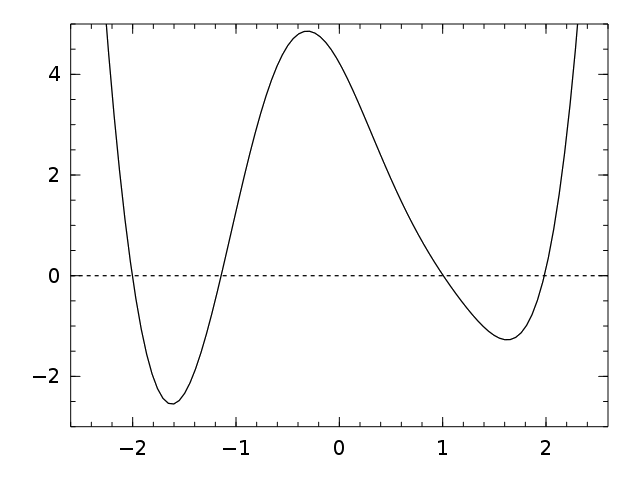
\includegraphics[height=0.6\textheight]{src/funex-1.png}
  \end{center}
  }
}

\subsection{Aproximação Linear}

\myframetop{
  \ctr{ Aproximação linear }
  \[ f(x) = f(a) + f'(a)(x-a) + E(x) \]
  \begin{center}
  \only<2>{ 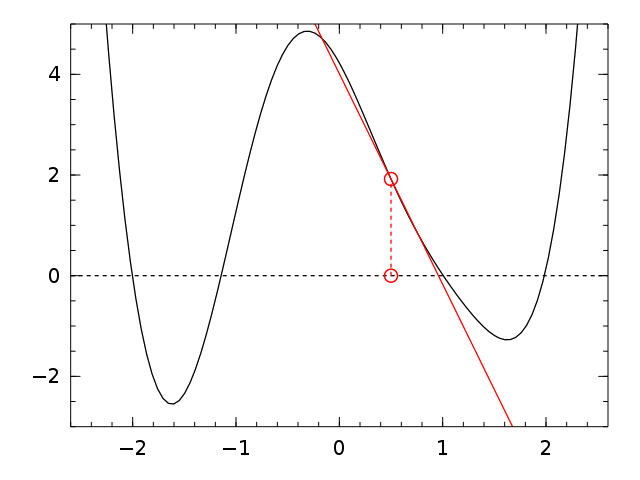
\includegraphics[height=0.6\textheight]{src/funex-2.png} }

  \only<3>{ 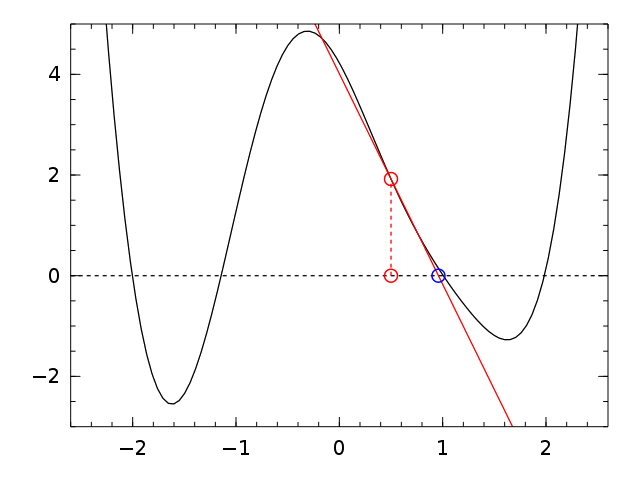
\includegraphics[height=0.6\textheight]{src/funex-3.png} }
  \end{center}
}

\myframe{
  \ctr{ O zero da função afim }
  \[ L(x) = f(a) + f'(a)(x-a) = 0 \]
  \pause
  \[ x = a - \frac{f(a)}{f'(a)}, \qquad
  f'(a) \neq 0 \]
}

\subsection{Método de Newton}

\myframe{
  \ctr{Método de Newton}
  Dado $x^0$, defina a sequência
  $$ x^{k+1} = x^k - \frac{f(x^k)}{f'(x^k)} $$
  se $f'(x^k) \neq 0$.

  \pause
  Sob {\bf hipóteses}, $f'(x^k) \rightarrow 0$.
}

\myframeout{
  \begin{center}
    \foreach \a in {1, 2, 3} {
      \foreach \b in {1,2,3} {
        \def\c{\the\numexpr3*\a+\b-3\relax}
        \only<\c>{ \includegraphics[height=0.8\textheight]{src/newton1d\a-s\b.png} }

      }

    }
  \end{center}
}


\section{Equações não-lineares}
\subsection{Introdução}

\myframetop{
  \ctr{Equações não-lineares}
  \begin{equation*}
    \left\{\begin{array}{rcl}
      x_1^2 + x_2^2 & = & 4 \\
      x_1x_2 & = & 1
    \end{array}\right.
  \end{equation*}
  \begin{equation*}
    \left\{\begin{array}{rcl}
      x_1^2 + x_2^2  - e^{x_1+x_2}& = & 1 \\
      \sqrt{1 + x_1^2} + \dfrac{1}{x_2^2 + 1} & = & 1
    \end{array}\right.
  \end{equation*}
  \begin{equation*}
    \left\{\begin{array}{rcl}
      x_1x_2x_3 & = & 1 \\
      x_1x_2 + x_1x_3 + x_2x_3 & = & 3 \\
      x_1 + x_2 + x_3 & = & 3
    \end{array}\right.
  \end{equation*}
}

\myframetop{
  \ctr{Equações não-lineares}
  $$ F(x) = 0, \qquad
  F:\mathbb{R}^n\rightarrow\mathbb{R}^n. $$
  \qquad
  \begin{equation*}
    \left\{\begin{array}{rcl}
      x_1^2 + x_2^2 & = & 4 \\
      x_1x_2 & = & 1
    \end{array}\right.
  \end{equation*}
  $$ F(x) = \left[\begin{array}{c}
      x_1^2 + x_2^2 - 4 \\ x_1x_2 - 1
  \end{array}\right]. $$
}

\myframetop{
  \ctr{Equações não-lineares}
  \begin{equation*}
    \left\{\begin{array}{rcl}
      \color{red} x_1^2 + x_2^2
      & \color{red} =
      & \color{red} 4 \\
      \color{blue} x_1x_2
      & \color{blue} =
      & \color{blue} 1
    \end{array}\right.
  \end{equation*}
  \begin{center}
    \begin{tikzpicture}[scale=0.8]
      \draw[->] (-2.6,0) -- (2.6,0);
      \draw[->] (0,-2.6) -- (0,2.6);
      \draw[red,thick] (0,0) circle (2);
      \draw[blue,thick,domain=0.4:2.5] plot (\x,{1/\x});
      \draw[blue,thick,domain=-2.5:-0.4] plot (\x,{1/\x});
      \only<2>{
        \fill (1.93,0.52) circle (0.08) --
              (0.52,1.93) circle (0.08) --
              (-1.93,-0.52) circle (0.08) --
              (-0.52,-1.93) circle (0.08);
      }
    \end{tikzpicture}
  \end{center}
}

\subsection{Aproximação Linear}

\myframetop{
  \ctr{A Aproximação linear}
  $$ F(x) \approx L(x) =  F(a) + F'(a)(x-a). $$
  \pause
  \begin{equation*}
    F(x) = \left[\begin{array}{c}
      x_1^2 + x_2^2 - 4 \\ x_1x_2 - 1
    \end{array}\right]
    \quad
    F'(x) = \left[\begin{array}{cc}
      2x_1 & 2x_2 \\ x_2 & x_1
    \end{array}\right]
    \quad
    a = \left[\begin{array}{c}
        2 \\ 1
    \end{array}\right].
  \end{equation*}
  \pause
  \begin{equation*}
    F(2,1) = \left[\begin{array}{c}
      1 \\ 1
    \end{array}\right]
    \quad
    F'(2,1) = \left[\begin{array}{cc}
      4 & 2 \\ 1 & 2
    \end{array}\right]
    \quad
  \end{equation*}
  \begin{equation*}
   L(x) =
    \left[\begin{array}{c}
      4x_1 + 2x_2 - 9 \\
      x_1 + 2x_2 - 3
    \end{array}\right].
  \end{equation*}
}

\myframetop{
  \ctr{Equações não-lineares}
  \begin{equation*}
    \left\{\begin{array}{rcl}
      \color{red} 4x_1 + 2x_2
      & \color{red} =
      & \color{red} 9 \\
      \color{blue} x_1 + 2x_2
      & \color{blue} =
      & \color{blue} 3
    \end{array}\right.
  \end{equation*}
  \begin{center}
    \begin{tikzpicture}[scale=0.8]
      \draw[->] (-2.6,0) -- (2.6,0);
      \draw[->] (0,-2.6) -- (0,2.6);
      \draw[red,thick,domain=1:2.5] plot (\x,{4.5 - 2*\x});
      \draw[blue,thick,domain=-1:2.5] plot (\x,{1.5 - 0.5*\x});
      \fill (2,1) circle (0.08);
      \draw[red,dashed] (0,0) circle (2);
      \draw[blue,dashed,domain=0.4:2.5] plot (\x,{1/\x});
      \draw[blue,dashed,domain=-2.5:-0.4] plot (\x,{1/\x});
      \only<2>{
        \fill (2,0.5) circle (0.08);
      }
    \end{tikzpicture}
  \end{center}
}

\myframe{
  \ctr{ A solução do sistema linear }
  \[ L(x) = F(a) + F'(a)(x - a) = 0, \] \pause
  $$ F'(a)(x-a) = -F(a), $$ \pause
  \[ x = a - [F'(a)]^{-1}F(a), \]
  $F'(a)$ não singular.
}

\subsection{Método de Newton}

\myframe{
  \ctr{O Método de Newton}
  Dado $x^0$, defina as sequências $\{d^k\}$ e $\{x^k\}$ por
  \[ F'(x^k)d^k = -F(x^k), \]
  \[ x^{k+1} = x^k + d^k, \]
  supondo-as bem definidas. \pause

  Sob {\bf hipóteses} $F(x^k) \rightarrow 0$.
}

\myframe{
  \ctr{O Método de Newton}
  \begin{align*}
    x^0 & = (2.00000, 1.00000), \qquad F(x^0) = (1.00000,  1.00000) \\
    x^1 & = (2.00000, 0.50000), \qquad F(x^1) = (0.25000,  0.00000) \\
    x^2 & = (1.93333, 0.51667), \qquad F(x^2) = (0.00472, -0.00111) \\
    x^3 & = (1.93185, 0.51764), \qquad F(x^3) = (0.00000, -0.00000)
  \end{align*}
  * Com 5 casas decimais
}

\section{Otimização}

\subsection{Introdução}

\myframe{
  \ctr{Otimização}
  $$ \min f(x), \qquad f:\mathbb{R}^n\rightarrow\mathbb{R}, f \in C^2 $$
  \pause
  \begin{description}
    \item<2->[CN1] Se $x^*$ é um minimizador local de $f$, então
      $\nabla f(x^*) = 0$.
    \item<3->[CN2] Se $x^*$ é um minimizador local de $f$, então
      $\nabla f(x^*) = 0$ e $\nabla^2 f(x^*)$ é semidefinida positiva.
    \item<4->[CS2] Se $\nabla f(x^*) = 0$ e $\nabla^2 f(x^*)$ é definida positiva,
      então $x^*$ é um minimizador local de $f$.
  \end{description}
}

\subsection{O Método de Newton}

\myframetop{
  \ctr{O Método de Newton para otimização}
  $$ F(x) = \nabla f(x) $$
  $$ F'(x) = \nabla^2 f(x) $$
  \pause
  $$ \nabla^2 f(x^k)d^k = -\nabla f(x^k) $$
  $$ x^{k+1} = x^k + d^k $$
}

\myframetop{
  \ctr{O Método de Newton para otimização}
  \only<1>{
    $$ \nabla^2f(x^k)d + \nabla f(x^k) = 0. $$
  }
  \only<2->{
    $$ \underbrace{\nabla^2f(x^k)d + \nabla f(x^k)}_{\nabla m(d)} = 0. $$
  }
  \only<3->{
    $$ m(d) = \frac{1}{2}d^T\nabla^2 f(x^k)d + \nabla f(x^k)^Td + f(x^k).$$
  }
  \only<4->{
    $$ d^k = \arg\min_d m(d). $$
    $$ x^{k+1} = \arg\min_x m(x-x^k). $$
  }
}

%\myframetop{
\myframeout{
  \ctr{O Método de Newton para otimização}
  $$ f(x) = (1-x_1)^2 + 4(x_2 - x_1^2)^2, \quad
  \only<1-3>{x^0 = (-0.500, 0.000)}
  \only<4-6>{x^1 = ( 0.000,-0.250)}
  \only<7-9>{x^2 = ( 0.333, 0.000)}
  \only<10-12>{x^3 = ( 0.686, 0.346)}
  \only<13-15>{x^4 = ( 0.843, 0.687)}
  \only<16-18>{x^5 = ( 0.974, 0.932)}
  \only<19-21>{x^6 = ( 0.997, 0.993)}
  $$
  \begin{center}
    \foreach \a in {1,2,3,4,5,6,7} {
      \foreach \b in {1,2,3} {
        \def\c{\the\numexpr3*\a+\b-3\relax}
        \only<\c>{ \includegraphics[height=0.6\textheight]{src/rosenbr\a-\b.png} }

      }

    }
  \end{center}
}

%\myframetop{
\myframeout{
  \ctr{O Método de Newton para otimização}
  \[ f(x) = x_1^3-3x_1 + x_2^2 \]
  \begin{center}
    \foreach \a in {1,2,3} {
      \foreach \b in {1,2,3} {
        \def\c{\the\numexpr3*\a+\b-3\relax}
        \only<\c>{ \includegraphics[height=0.6\textheight]{src/min-newton-works\a-\b.png} }

      }

    }
  \end{center}
}

%\myframetop{
\myframeout{
  \ctr{O Método de Newton para otimização}
  \[ f(x) = x_1^3-3x_1 + x_2^2 \]
  \begin{center}
    \foreach \a in {1,2,3} {
      \foreach \b in {1,2,3} {
        \def\c{\the\numexpr3*\a+\b-3\relax}
        \only<\c>{ \includegraphics[height=0.6\textheight]{src/min-newton-fail\a-\b.png} }

      }

    }
  \end{center}
}

\section{Convergência}

\subsection{Convergência}

\foreach \ex in {1,2} {
\myframe{
  \[ f(x) = x^2 - 1 \]
  \begin{center}
    \foreach \a in {1,2,3} {
      \foreach \b in {1,2,3} {
        \def\c{\the\numexpr3*\a+\b-3\relax}
        \only<\c>{ \includegraphics[height=0.8\textheight]{src/conv1d-ex\ex-\a-s\b.png} }

      }

    }
  \end{center}
}
}

\myframe{
  $$ f(x) = x^2 - 1 $$
  \begin{center}
    \foreach \a in {1, 2, 3} {
      \only<\a>{ \includegraphics[height=0.8\textheight]{src/conv-ex1-\a.png} }

    }
  \end{center}
}


\foreach \ex in {3,4,5,6,7,8,9} {
\myframe{
  \[ f(x) = x^3 - x \]
  \begin{center}
    \foreach \a in {1,2,3} {
      \foreach \b in {1,2,3} {
        \def\c{\the\numexpr3*\a+\b-3\relax}
        \only<\c>{ \includegraphics[height=0.8\textheight]{src/conv1d-ex\ex-\a-s\b.png} }

      }

    }
  \end{center}
}
}

\myframe{
  $$ f(x) = x^3 - x $$
  \begin{center}
    \foreach \a in {1, 2, 3, 4, 5} {
      \only<\a>{ \includegraphics[height=0.8\textheight]{src/conv-ex2-\a.png} }

    }
  \end{center}
}

\myframe{
  \ctr{Em duas dimensões}
  \begin{equation*}
    \left\{\begin{array}{rcl}
      x_1^2 + x_2^2 & = & 4 \\
      x_1x_2 & = & 1
    \end{array}\right.
  \end{equation*}
  \begin{minipage}{0.48\textwidth}
    \begin{center}
    \begin{tikzpicture}[scale=1.0]
      \draw[->] (-2.6,0) -- (2.6,0);
      \draw[->] (0,-2.6) -- (0,2.6);
      \draw (-2,-2) rectangle (2,2);
      \draw[black,thick] (0,0) circle (2);
      \draw[black,thick,domain=0.4:2.5] plot (\x,{1/\x});
      \draw[black,thick,domain=-2.5:-0.4] plot (\x,{1/\x});
      \fill[red] (1.93,0.52) circle (0.08);
      \fill[green] (0.52,1.93) circle (0.08);
      \fill[yellow] (-1.93,-0.52) circle (0.08);
      \fill[blue] (-0.52,-1.93) circle (0.08);
    \end{tikzpicture}
    \end{center}
  \end{minipage}
  \begin{minipage}{0.48\textwidth}
    \only<1>{ 
\includegraphics[height=0.46\textheight]{src/ex1.png} }

    \only<2>{ 
\includegraphics[height=0.46\textheight]{src/ex3.png} }
  \end{minipage}
}

\myframe{
  \ctr{O exemplo tradicional}
  $$ z^3 = 1, \qquad z \in \mathbb{C} $$
  $$ z = 1, \frac{-1+\sqrt{3}i}{2}, \frac{-1-\sqrt{3}i}{2}. $$
  \begin{center}
    \begin{tikzpicture}[scale=0.8]
      \draw[->] (0,-1.6) -- (0,1.6) node[left] {Imag.};
      \draw[->] (-1.6,0) -- (1.6,0) node[below] {Real};
      \fill (1,0) circle (0.08);
      \fill (-0.5,-0.866) circle (0.08);
      \fill (-0.5, 0.866) circle (0.08);
    \end{tikzpicture}
  \end{center}
}

\myframe{
  \ctr{O exemplo tradicional}
  $$ z = x + yi $$
  $$ z^3 = (x^3-3xy^2) + (3x^2y-y^3)i $$
  \begin{equation*}
    F(x,y) = \left[
    \begin{array}{c}
      x^3 - 3xy^2 - 1 \\ 3x^2y-y^3
  \end{array}\right]
  \end{equation*}
}

\myframe{
  \only<1>{
    \ctr{O exemplo tradicional}
  }
  \only<2->{
    \ctr{O fractal de Newton}
  }
  \begin{center}
    \only<1-2>{
      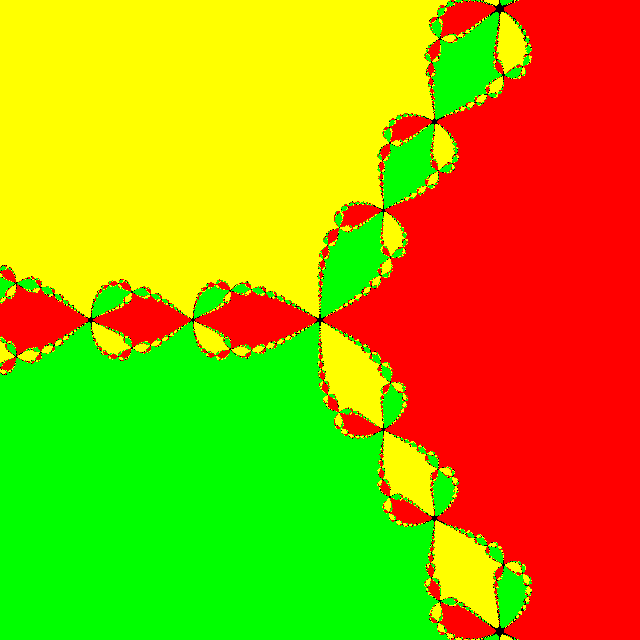
\includegraphics[height=0.7\textheight]{src/ex2.png}
    }
    \only<3>{
      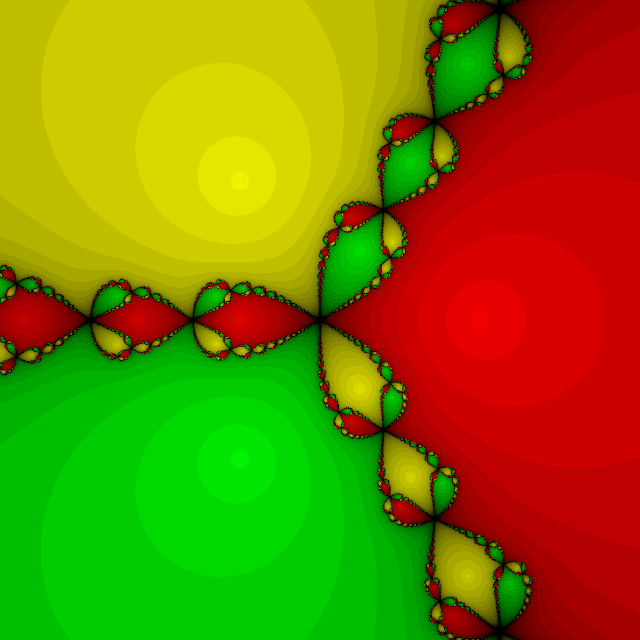
\includegraphics[height=0.7\textheight]{src/ex4.png}
    }
  \end{center}
}

\myframe{
  \begin{equation*}
    F(x,y) = \left[
    \begin{array}{c}
      x(y-x^2) \\ (x^2-1)(y+1)
  \end{array}\right]
  \end{equation*}
  \begin{center}
    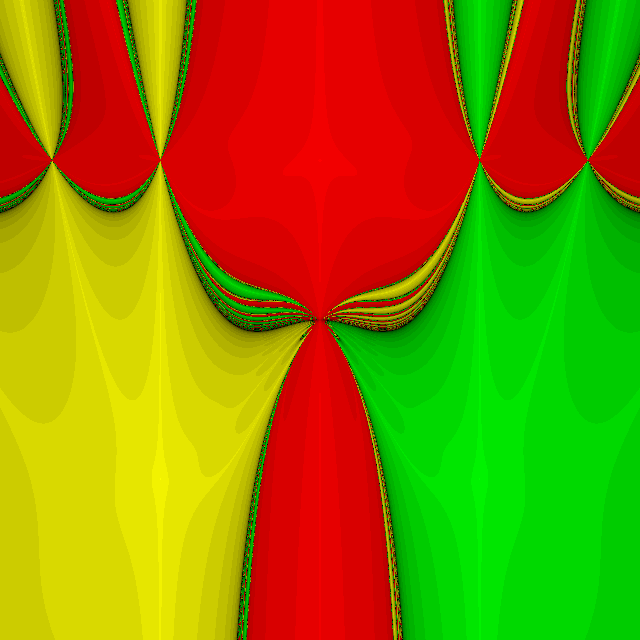
\includegraphics[height=0.7\textheight]{src/ex5.png}
  \end{center}
}

\myframe{
  \begin{equation*}
    z^4 = 1, \qquad z \in \mathbb{C}
  \end{equation*}
  \begin{center}
    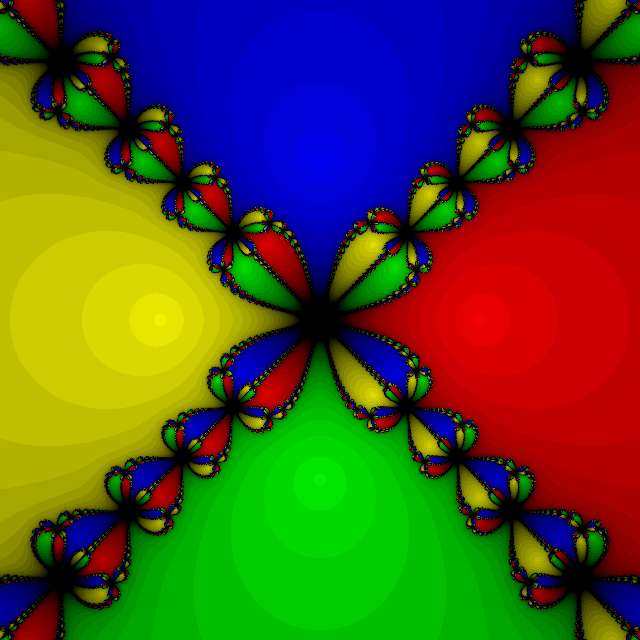
\includegraphics[height=0.7\textheight]{src/ex6.png}
  \end{center}
}


\myframe{
  \hfill
  \begin{beamercolorbox}[center, wd=0.6\textwidth, rounded=true,
      shadow=true]{secbox}
    \bf \LARGE \thanksmsg
  \end{beamercolorbox}
  \hfill{}

  \begin{center}
    \includegraphics[scale=0.7]{img/cc.png} \qquad
    \includegraphics[scale=0.7]{img/by.png} \qquad
    \includegraphics[scale=0.7]{img/sa.png}

  \ifpt{
    Esta apresentação está licenciada com uma Licença Creative Commons
    Atribuição-CompartilhaIgual 4.0 Internacional.
  }\else{
    This presentation is licensed under the Creative Commons Attributions-ShareAlike 4.0
    International License.
  }\fi
  \end{center}
}

\end{document}
